\chapter{Magnetic Field in Matter}
\section{Magnetization}
\begin{wrapfigure}{r}{0.3\textwidth}
	\begin{center}
		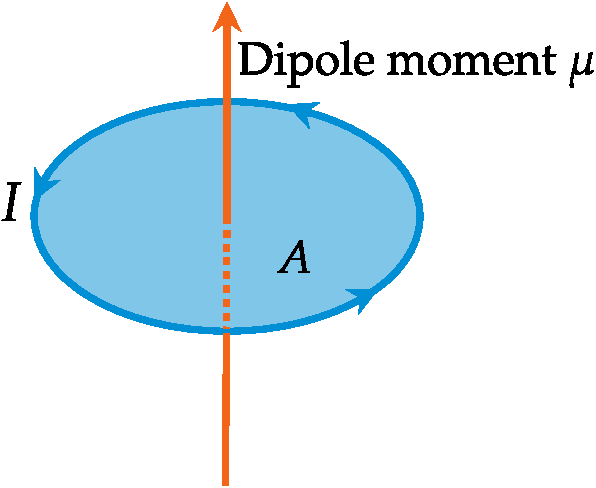
\includegraphics[width=0.28\textwidth]{magnetic moment}
	\end{center}
	\caption{magnetic dipole moment}
\end{wrapfigure}

In  electrostatics, we had seen that the electrical polarization of the medium  influences the electrical behavior of substances. In the same way we have internal currents within a material because there are moving charges in atoms and molecules which can create their own magnetic field.Any current loop has a magnetic field and thus has a magnetic dipole moment.There are two types effects here, the first is due to the orbital motion of the electrons and the second is due to the intrinsic spin magnetic moment of the electrons. The second effect is purely quantum mechanical in origin .Like in the electrostatic case, the magnetic moment could be intrinsic to an atom or molecule or it could be induced by an externally applied magnetic field. \par
Ordinarily, the current loops inside an object cancel each other out because of the random orientation of the atoms. But when a magnetic field is applied, a net alignment of these magnetic dipoles occurs, and the medium becomes magnetically polarized, or magnetized.
\\
Let ${m_{i}}$ be the magnetic moment of the $\mathrm{i}$ -th atom inside a matter. We define magnetization as the net magnetic moment per unit volume
$$
\vec{M}=\lim _{\Delta V \rightarrow 0} \frac{\sum_{i} {m_{i}}}{\Delta V}
$$
The magnetization  plays a role analogous to the polarization ${P}$ in electrostatics.  The magnetization  could be paramagnetism, diamagnetism, or even ferromagnetism. We'll discuss it later.
\subsection{Surface and Volume current}
Suppose we have a piece of magnetized material the magnetic dipole moment per unit volume, ${M}$, is given.The vector potential of a single dipole ${m}$ is given by, (We don't do derivation here).
\begin{align*}
\vec{\mathrm{A}}(\mathrm{r})&=\frac{\mu_{0}}{4 \pi} \int \frac{1}{r}\left[\nabla^{\prime} \times \mathrm{M}\left(\mathrm{r}^{\prime}\right)\right] \mathrm{d} \tau^{\prime}+\frac{\mu_{0}}{4 \pi} \oint \frac{1}{\mathrm{r}}\left[\vec{\mathrm{M}}\left(\mathrm{r}^{\prime}\right) \times \vec{\mathrm{d}} \mathrm{a}^{\prime}\right]
\intertext{The first term looks like the potential of a volume current density,}
{J}_{M}&=\nabla \times {M},
\intertext{While the second term looks like the potential of a surface current density,}
{K}_{M}&={M} \times \hat{n}
\intertext{Where $\hat{n}$ is the normal unit vector. With these definitions,}
\vec{A}({r})&=\frac{\mu_{0}}{4 \pi}\left\{\int \frac{{J}_{M}\left({r}^{\prime}\right)}{r} d\tau^{\prime}+\oint \frac{{K}_{M}\left({r}^{\prime}\right)}{r} \vec{d a^{\prime}}\right\}
\end{align*}
\subsection{Auxiliary Field}
There are both free and bound current in a magnetic material. So the total current ${J}$ could be written as
\begin{align*}
\vec{J}&=\mathrm{J}_{\mathrm{b}}+\mathrm{J}_{\mathrm{f}}
\intertext{Where ${J}_{b}$ is bound and ${J}_{f}$ is the free current.}
\intertext{According to Ampere's law,}
\oint \vec{\mathrm{B}} \cdot \mathrm{d} \vec{l}&=\mu_{0} \mathrm{I}_{\mathrm{enc}} \\
\vec{\nabla} \times \vec{\mathrm{B}}&=\mu_{0} \vec{\mathrm{J}}
\intertext{ Let us substitute the value of $J_b$}
\vec{\mathrm{J}}_{\mathrm{b}}&=\vec{\nabla} \times \vec{\mathrm{M}} \\
\frac{1}{\mu_{0}}(\vec{\nabla} \times \vec{\mathrm{B}})&=\vec{\mathrm{J}}\\&=\vec{\mathrm{J}}_{\mathrm{f}}+\vec{\mathrm{J}}_{\mathrm{b}}\\&=\vec{\mathrm{J}}_{\mathrm{f}}+(\vec{\nabla} \times \vec{\mathrm{M}}) \\
\vec{\nabla} \times\left(\frac{1}{\mu_{0}} \vec{\mathrm{B}}-\vec{\mathrm{M}}\right)&=\vec{\mathrm{J}_{\mathrm{f}}}
\intertext{Now, define the quantity inside the curl as ${H}$}
\vec{\mathrm{H}} &\equiv \frac{1}{\mu_{0}} \vec{\mathrm{B}}-\vec{\mathrm{M}}
\intertext{So now the equation becomes}
\vec{\nabla} \times \overrightarrow{\mathrm{H}}&=\overrightarrow{\mathrm{J}}_{\mathrm{f}}
\intertext{Or in integral terms,}
\phi \overrightarrow{\mathrm{H}} \cdot \mathrm{d} \vec{l}&=\mathrm{I}_{\mathrm{fenc}}
\intertext{Where $I_{\text {fenc }}$ is the total free current passing through the Amperian loop. These are the forms of Ampere's law inside matter. $  H $ plays a role in magnetostatics analogous to $D$ in electrostatics:}
\end{align*}
\section{Linear and Non linear medium}
To complete the description of macroscopic magnetostatics, there must be a constitutive relation between ${H}$ and ${B}$.
\begin{align}
\notag {M}&\propto{H}\\
{M}&=\chi_{m} {H}\label{magnetic susceptibility}
\end{align}
 The constant $\chi_{m}$ is called the magnetic susceptibility. It is dimensionless quantity it's typical values are around $10^{-5}$.
 Materials that obey equation.\ref{magnetic susceptibility} are called linear media. For linear media
 \begin{align*}
 {B}&=\mu_{0}({H}+{M})=\mu_{0}\left(1+\chi_{m}\right) {H}
 \intertext{ Thus ${B}$ is also proportional to ${H}$ :}
 {B}&=\mu {H}
  \intertext{Where $\mu=\mu_{0}\left(1+\chi_{m}\right)$ is the permeability of the material.}
\end{align*}
 \section{Diamagnetism, Paramagnetism, Ferromagnetism}
Based on the magnetic response, materials can be classified into the following three major groups:  Diamagnetism,  Paramagnetism,  and Ferromagnetism.
\subsection{Diamagnetism} 
Diamagnetism, a very weak fundamental property of all matter, arises due to the non-cooperative behavior of orbiting electrons when exposed to an externally applied magnetic field. 
\begin{itemize}
	\item  Very weak; exists ONLY in presence of an external field, non-permanent.
	\item  Applied external field acts on atoms of a material, slightly unbalancing their orbiting electrons, and creates small magnetic dipoles within atoms which oppose the applied field. This action produces a negative magnetic effect known as diamagnetism.
	\item  The induced magnetic moment is small, and the magnetization $(M)$ direction is opposite to the direction of applied field $(H)$.
	\item  Thus the relative permeability is less than unity i.e. magnetic susceptibility $(\chi_{m})$ is negative, and is in order of $-10^{-5}$.
	\item  Materials such as $\mathrm{Cu}, \mathrm{Ag}, \mathrm{Si}$, Ag and alumina are diamagnetic at room temperature.
\end{itemize}
\subsection{Paramagnetism} 
Materials which exhibit a small positive magnetic susceptibility in the presence of a magnetic field are called para-magnetic, and the effect is termed as para-magnetism.
This class of the materials has a net magnetic moment due to the existence of unpaired electrons in partially filled orbitals. However, the individual magnetic moments do not interact magnetically and hence the magnetization is zero when there is no external applied field or when the externally applied field is removed.
\begin{itemize}
	\item  Slightly stronger than Diamagnetism. When an external field is applied dipoles line-up with the field, resulting in a positive magnetization. However, the dipoles do not interact.
	 
	\item In the absence of an external field, the orientations of atomic magnetic moments are random leading to no net magnetization.
	\item  When an external field is applied dipoles line-up with the field, resulting in a positive magnetization.
	- However, because the dipoles do not interact, extremely large magnetic fields are required to align all of the dipoles.
	\item  In addition, the effect is lost as soon as the magnetic field is removed.
	\item  Since thermal agitation randomizes the directions of the magnetic dipoles, an increase in temperature decreases the paramagnetic effect.
	\item Magnetic susceptibility $(\chi_{m})$  of these materials is slightly positive, and lies in the range $+10^{-5}$ to $+10^{-2}$
	\item  Para-magnetism is produced in many materials like aluminium, calcium, titanium, alloys of copper.
\end{itemize}

\subsection{Ferromagnetism} 
Certain materials possess permanent magnetic moments even in the absence of an external field, These are called Ferromagnetic materials.
The atomic moments in these materials exhibit very strong interactions. These interactions are produced by electronic exchange forces and result in either a parallel or an antiparallel alignment of atomic moments 
\begin{itemize}
	\item  Both dia- and para- magnetic materials are considered as non-magnetic because they exhibit magnetization only in presence of an external field.

\item  The permennat dipoles can easily line-up with the imposed magnetic field due to the exchange interaction or mutual reinforcement of the dipoles. These are chrematistics of ferromagnetism.
\item  Materials with ferro-magnetism (Examples: Fe, Co, Ni, Gd) possess magnetic susceptibilities approaching $10^{6}$.
	\item  Above a specific temperature called Curie temperature, ferro-magnetic materials behave as para-magnetic materials and their susceptibility is given by the Curie-Weiss law, defined as
	$$
	\chi_{m}=\frac{C}{T-T_{c}}
	$$
	 Where $C$ - material constant, $T-$ temperature, $T_{c}-$ Curie temperature.
	\item  Ferro Magnets are very strong; dipoles line-up permanently upon application of external field. Has two sub-classes:-
	\begin{itemize}
		\item Anti-ferro-magnetism.
		\item  Ferri-magnetism
	\end{itemize}
	
\end{itemize}
 \section{Magnetostatic Boundary Conditions}
Just as the electric field suffers a discontinuity at a surface charge, so the magnetic field is discontinuous at a surface current. Only this time it is the tangential component that changes.
\begin{figure}[H]
	\centering
	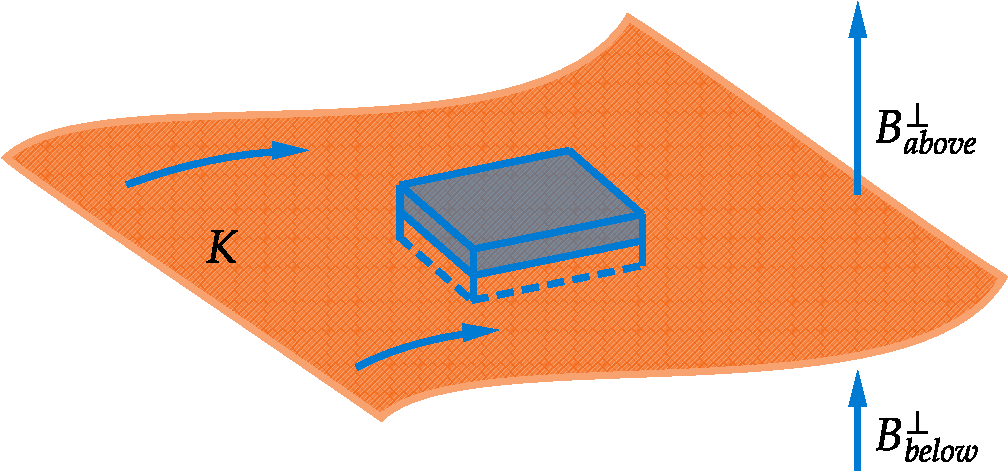
\includegraphics[height=4cm,width=6.5cm]{3-crop}
	\caption{Wafer thin pillbox}
	\label{Wafer thin pillbox}
\end{figure}
 Indeed, if we apply $\nabla \cdot {B}=0$ in the integral form
$\oint_{S} {B} \cdot  d a=0$\ 
to a thin gaussian pillbox straddling the surface Figure. \ref{Wafer thin pillbox} , we obtain,
\begin{equation}\label{boundary condition}
B_{above}^{\perp}-B_{below}^{\perp}=0.
\end{equation}
Where $B^{\perp}$ is the component of the magnetic field ${B}$ perpendicular to the surface. Equation.\ref*{boundary condition} tells us that
$B^{\perp}$ is continuous at the interface. 
\begin{figure}[H]
	\centering
	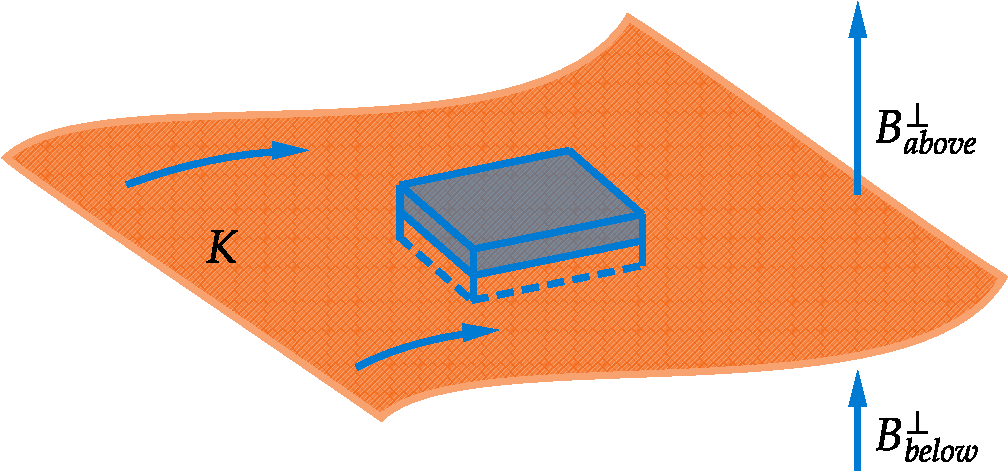
\includegraphics[height=4cm,width=6.5cm]{3-crop}
	\caption{Amperian loop}
	\label{Amperian loop}
\end{figure}
\begin{align}
\intertext{As for the tangential components, from Ampere's law $\nabla \times {B}=\mu_{0}{I_{enc}}$ an amperian loop running perpendicular to the current figure.\ref{Amperian loop} yields}
\notag \oint {B} \cdot d {l}&=\left(B_{above}^{\|}-B_{below}^{\|}\right) l\\\oint {B} \cdot d {l}&=\mu_{0}K l .\\
\text{or} \quad B_{above}^{\|}-B_{below}^{\|}&=\mu_{0}K
\intertext{Thus the component of ${B}$ that is parallel to the surface but perpendicular to the current is discontinuous in the amount $\mu_{0}K$.These results can be summarized in a single formula: }
\vec{\mathrm{B}}_{\text {above }}-\vec{\mathrm{B}}_{\text {below }}&=\mu_{0}(\mathrm{~K} \times \hat{\mathrm{n}})
\intertext{Where $\hat{n}$ is a unit vector perpendicular to the surface, pointing "upward". Like the scalar potential of electrostatics the magnetic vector potential is also continuous}
A_{\text {above }}&=A_{\text {below }}
\intertext{But the derivative of vector potential has a discontinuity}
\frac{\partial \mathrm{A}_{\mathrm{above}}}{\partial \mathrm{n}}-\frac{\partial \mathrm{A}_{\text {below }}}{\partial \mathrm{n}}&=-\mu_{0} \mathrm{~K}
\end{align}
\begin{center}
	\framebox{
		\parbox[t][6cm]{7cm}{
			
			\addvspace{0.2cm} \centering 
			\begin{align*}
			B_{above}^{\perp}-B_{below}^{\perp}&=0\\\\
			B_{above}^{\|}-B_{below}^{\|}&=\mu_{0}K\\\\
			A_{\text {above }}&=A_{\text {below }}\\\\ \frac{\partial \mathrm{A}_{\mathrm{above}}}{\partial \mathrm{n}}-\frac{\partial \mathrm{A}_{\text {below }}}{\partial \mathrm{n}}&=-\mu_{0} \mathrm{~K}
			\end{align*}
			} }
\end{center}
\newpage
\begin{abox}
	Previous year solutions
	\end{abox}
\begin{enumerate}
	\begin{minipage}{\textwidth}
		\item At a surface current, which one of the magnetostatic boundary condition is $\underline{\text { NOT }}$ CORRECT?
		\exyear{GATE 2013}
	\end{minipage}
	\begin{tasks}(1)
		\task[\textbf{A.}] Normal component of the magnetic field is continuous.
		\task[\textbf{B.}]Normal component of the magnetic vector potential is continuous.
		\task[\textbf{C.}]Tangential component of the magnetic vector potential is continuous.
		\task[\textbf{D.}]Tangential component of the magnetic vector potential is not continuous.
	\end{tasks}
	\begin{answer}
		THe correct option is \textbf{(d)}
	\end{answer}

\end{enumerate}

